%%% XeLaTeX-article %%%
%# -*- coding: utf-8 -*-
%!TEX encoding = UTF-8 Unicode
%!TEX TS-program = xelatex  
%---------------------虽然加了%还是要保留!

\documentclass[17pt]{beamer}
\mode<presentation>
{
\usetheme[width=40pt]{Hannover}
\usecolortheme[]{dove}
\usefonttheme[]{structurebold}
\setbeameroption{hide notes}
}

\usepackage{fontspec}
\setmainfont{Arial} %设置主字体
\newfontfamily\sanskritfont[Script=Devanagari,Mapping=romantodevanagari,Scale=1.15]{Sanskrit 2003}             %输出天城体
%\newfontfamily\sanskritfont[Mapping=tex-text]{Times New Roman}              %输出转写
\doublehyphendemerits=-10000
\newcommand{\skt}[1]{{\sanskritfont{#1}}} %输出天城体
\newcommand{\skttrans}[1]{{\skt{#1}~#1}}  %输出天城体和转写
%----------------------------------------------------设置梵文输入方法

\usepackage[UTF8,fontset=windows]{ctex}
\usepackage{amsmath}
%----------------------------------------------------设置中文环境

\usepackage{graphicx}
\usepackage{flafter} 
\graphicspath{{pic/}}
\usepackage{booktabs} 
%-----------------------------------------插图表格

\usepackage{hyperref} 
\hypersetup{
    colorlinks=true,
    linkcolor=black,
    urlcolor=blue
}
\usepackage{xcolor}
%------------------------------颜色


\title{{梵语入门}}
\subtitle{2. 梵语字母}
\author[张雪杉]{文学院~~张雪杉 \\ zhangxueshan@sdnu.edu.cn}
\date{}
%\institute{}



\begin{document}	


\begin{frame}
  \titlepage
\end{frame}

\begin{frame}
  \frametitle{本节内容}
  \tableofcontents
\end{frame}

\section{课程介绍}
\begin{frame}{\insertsection }  
  \includegraphics[width=0.7\textwidth]{Course_intro.png} %
  \begin{itemize}
    \item
      超星学习通课程邀请码:1855857
    \item
      新选课同学请自行查看第一周ppt
  \end{itemize}
\end{frame}

\subsection{上节问题}
\begin{frame}{\insertsubsection ~~ 手写字体}  
  \centering
  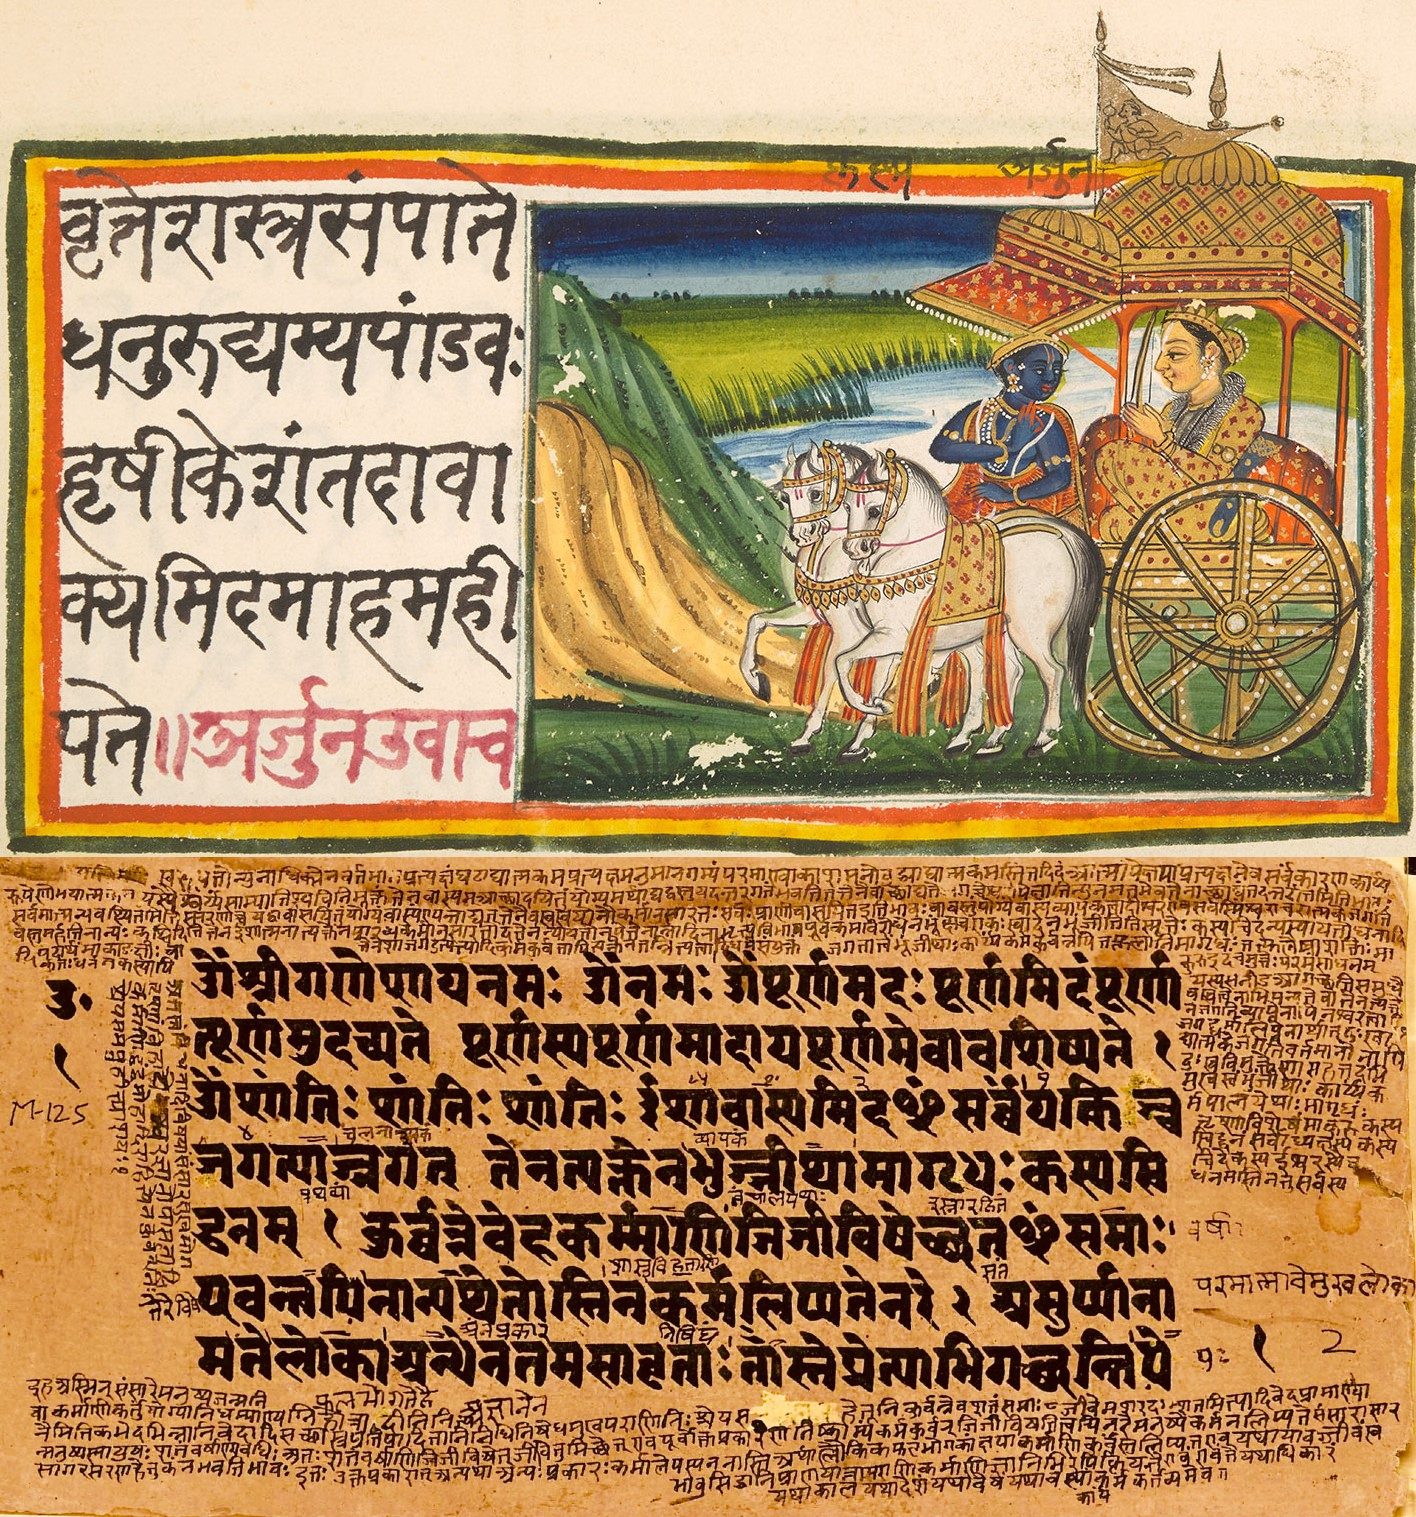
\includegraphics[width=0.7\textwidth]{handwriting.png} %
\end{frame}

\section{梵语字母}
\begin{frame}{\insertsection }
    \tableofcontents[currentsection]
\end{frame}

\subsection{元音}

\begin{frame}{\insertsubsection ~~ 独立形式}
  %\small
  \begin{itemize}
    \item
      字母排列总则:发音部位从后往前
    \item
      元音的独立形式:出现在词首
  \end{itemize}
  \bigskip

    \begin{tabular}{@{}llllllll@{}} % 7 columns: type, length/type, and 5 vowels
      简单元音 & \skttrans{a} & \skttrans{ā} & \skttrans{i} & \skttrans{ī} & \skttrans{u} & \skttrans{ū} \\
       & \skttrans{ṛ} & \skttrans{ṝ} & \skttrans{ḷ} & & & \\
    \end{tabular}

    复合元音 ~\skttrans{e} ~\skttrans{ai} ~\skttrans{o} ~\skttrans{au}
\end{frame}

\begin{frame}{\insertsubsection ~~ 附属形式}
  \begin{itemize}
    \item
      元音的附属形式:辅音之后
  \end{itemize}
  \centering
  \begin{tabular}{@{}llllll@{}} % 6 columns
    \skttrans{ka} & \skttrans{ki} & \skttrans{ku} & \skttrans{kṛ} & \skttrans{kḷ}   \\
    \skttrans{kā} & \skttrans{kī} & \skttrans{kū} & \skttrans{kṝ} &  \\
    & \skttrans{ke} & \skttrans{ko} &  & \\
    & \skttrans{kai} & \skttrans{kau} &  & \\
    \skttrans{'} & \skttrans{kaṃ} & \skttrans{kaḥ} &  & \skttrans{k} \\
    特殊 & \skttrans{hṛ} & \skttrans{ru} & \skttrans{rū} &  \\
  \end{tabular}
\end{frame}

\subsection{辅音}

\begin{frame}{发音部位}
  \centering    
  \includegraphics[width=0.9\textwidth]{placeofarticulation.png}
\end{frame}

\begin{frame}{发音部位}
  \centering    
  \includegraphics[width=0.8\textwidth]{placeofarticulation4varga.png}
\end{frame}

\begin{frame}{\insertsubsection ~~ 字母顺序}
  \small
  \begin{tabular}{@{}llllll@{}} % 6 columns
     & 不送气  & 送气 & 不送气 & 送气 &   \\
     & 清音  & 清音 & 浊音 & 浊音 & 鼻音  \\
    喉音  & \skttrans{ka}  & \skttrans{kha} & \skttrans{ga} & \skttrans{gha} & \skttrans{ṅa} \\
    腭音  & \skttrans{ca}  & \skttrans{cha} & \skttrans{ja} & \skttrans{jha} & \skttrans{ña} \\
    顶音  & \skttrans{ṭa}  & \skttrans{ṭha} & \skttrans{ḍa} & \skttrans{ḍha} & \skttrans{ṇa} \\
    齿音  & \skttrans{ta}  & \skttrans{tha} & \skttrans{da} & \skttrans{dha} & \skttrans{na} \\
    唇音  & \skttrans{pa}  & \skttrans{pha} & \skttrans{ba} & \skttrans{bha} & \skttrans{ma} \\
      &  & &  & &   \\
    半元音  & \skttrans{ya}  & \skttrans{ra} & \skttrans{la} & \skttrans{va} &  \\
    咝音  & \skttrans{śa}  & \skttrans{ṣa} & \skttrans{sa} &  \skttrans{ha} & \\
  \end{tabular}
\end{frame}

\begin{frame}{\insertsubsection ~~ 发音部位}
    \centering    
    \includegraphics[width=\textwidth]{consonant_system.png}
\end{frame}

\begin{frame}{复合辅音}
  \small
  {\centering
    \begin{tabular}{@{}lllll@{}} % 7 columns: type, length/type, and 5 vowels
      左右连 & \skttrans{tva}  & \skttrans{tma} & \skttrans{sya} & \skttrans{ṣya} \\
      & \skttrans{tma}  & \skttrans{nti} & \skttrans{bhya} & \skttrans{ṣṭa}   \\
      上下连  & \skttrans{dva}  & \skttrans{dda} & \skttrans{ṅga} & \skttrans{ddho} \\
      r在前 & \skttrans{rpa}  & \skttrans{rmya} & \skttrans{ryāṃ} & \skttrans{rgo} \\
      r在后  & \skttrans{pra}  & \skttrans{gra} & \skttrans{sra} & \skttrans{dra} \\
      特殊  & \skttrans{kṣa}  & \skttrans{jña} & \skttrans{kta} & \skttrans{tta} \\
        & \skttrans{dma}  & \skttrans{ddhya} & \skttrans{śva} & \skttrans{śca} \\
        & \skttrans{hma}  & \skttrans{hva} & \skttrans{hṇa} & \skttrans{tra} \\
    \end{tabular}
  }
  \begin{itemize}
    \item
      识读顺序:从左往右,从上往下
  \end{itemize}
\end{frame}

\subsection{字母相关资源}
\begin{frame}{\insertsubsection }
  \begin{itemize}
    \item
      课本第366-372页附录1
    \item
      \href{https://hindibhasha.com/hindiscripttutor.htm}{课本推荐的练习网站 by SOAS}
    \item
      多邻国软件印地语课程字母部分
    \item 
      课程相关资源 

      \begin{itemize}
        \item
          \href{https://www.youtube.com/playlist?list=PLWC1FN5zLbvrvsTc2zYyk5rumP-7R55Bw}{教材配套网课}
        \item
          其他网课(收费免费都有,

          微信公众号:僧言僧语)
        \item
          其他教材(要注意做练习)
      \end{itemize}
  \end{itemize}
\end{frame}  


\subsection{字母练习}
\begin{frame}{\insertsubsection ~~第一章练习1}
  \centering
  \begin{tabular}{@{}lllllll@{}} % 6 columns
    a) & \skt{ta}  & \skt{ka}  & \skt{pha} & \skt{pa} & \skt{ṣa} & \skt{a}  \\
    & \skt{ma}  & \skt{ca}  & \skt{tha} & \skt{na} & \skt{i} & \skt{ra}  \\
    b) & \skt{sa}  & \skt{ma}  & \skt{śa} & \skt{ṛ} & \skt{u} & \skt{ū}  \\
    & \skt{ja}  & \skt{pha}  & \skt{ba} & \skt{bha} & \skt{na} & \skt{ta}  \\
    c) & \skt{ṣa}  & \skt{va}  & \skt{ha} & \skt{ṭa} & \skt{ṅa} & \skt{ī}  \\
    & \skt{bha}  & \skt{dha}  & \skt{gha} & \skt{ai} & \skt{la} & \skt{sa}  \\
    d) & \skt{au}  & \skt{gha}  & \skt{la} & \skt{ta} & \skt{na} & \skt{tha}  \\
    & \skt{ya}  & \skt{dha}  & \skt{ba} & \skt{va} & \skt{śa} & \skt{ṣa}  \\
  \end{tabular}
\end{frame}

\section{本节作业}

\begin{frame}{\insertsection }
  \begin{itemize}
    \item
      第一章练习3
    \item
      阅读教材第0-2课相关内容
    \bigskip
    \item
      现在请做学习通\nobreakdash-章节\nobreakdash-课后问卷
  \end{itemize}
\end{frame}  

\end{document}	
